%\section{Integration and Test Facility (ITF)}
\section{Integrating the APA, CE and PD Systems}
%\label{sec:fdsp-tc-itf}
\label{sec:fdsp-tc-apa-integ}

% pgraph not needed. Anne. This section describes the baseline plan to assemble the \dword{apa}, \dword{ce}, and \dword{pd} in a surface facility. The installation team is investigating in parallel the possibility of performing the work underground. A decision will be made as to what is the optimal course of action prior to the TDR being finalized.

%The components of the \dword{dune} detectors will be manufactured in several different countries. Many of the parts can be reasonably shipped to the logistics warehouse and then underground where it can be installed. However, the  \dword{ce} and the \dwords{pd} are tightly coupled to the \dword{apa}s. The wires and filters on the \dword{apa}s form part of the electronics circuit, and the photon supports and cabling are built into the \dword{apa}s. Integrating the \dword{ce} and \dword{pd}s into the \dword{apa}s is a large task.  The present plan is integrate and test the components as early in the process as possible in a surface facility.  To avoid creating integration testing facilities at each factory, one central facility will be established in South Dakota near the \dword{surf} site. The \dword{apa}s, \dword{ce}, and \dwords{pd} modules will arrive in this \dword{itf}, undergo initial tests, be integrated, and then undergo a set of warm tests. 

The  \dword{ce} and the \dwords{pd} are tightly coupled to the \dword{apa}s, with the wires and filters on the \dword{apa}s forming part of the electronics circuit, and the \dword{pd} supports and cabling built into the frames. Integrating the \dword{ce} and \dwords{pd} into the \dword{apa}s is a large task.  This section describes the baseline plan to assemble these components underground.  

%The present plan is to integrate and test these subsystems as early in the process as possible in a surface facility.  We will establish a central \dword{itf} in South Dakota near the \dword{surf} site for this purpose. 
The \dword{apa}s, \dword{ce}, and \dwords{pd} modules will arrive independently first at the \dword{sdwf}, then to the Ross Headframe, according to the logistics scheduling. After transport  underground, the components will undergo initial tests, integration, and once integrated, a set of warm tests. %They will be repackaged for intermediate shipment to the \dword{sdwf} or direct shipment to \dword{surf}, depending on space availability.
\fixme{check my edits. anne}

%Because the \dword{ce} will be available approximately two years before installation begins, the \dword{itf} must be available on the same timescale. Other components are, in fact, available earlier. 
%The last of these subsystems, the \dword{ce}, 
The \dword{ce} is currently expected to be the last of these subsystems to be ready. The \dword{ce} components will be available approximately two years before detector installation begins. %, therefore the \dword{itf} must be available on the same timescale. 
Table \ref{tab:specs:just:SP-TC} summarizes the specifications for the %\dword{itf}
integration area;  SP-TC-5 and SP-TC-6.
%the relevant specifications involve the quality of the cleanroom and the UV light filtering for the \dwords{pd}.



%\begin{dunetable}
%[ITF Specifications]
%{cc}
%{tab:tcps-itf-spec}
%{Summary of the high level specifications for the ITF. %The building requirements are covered separately in a separate section.}
%Parameter & Specification \\ \toprowrule
%Cleanroom & The ITF cleanroom shall meet ISO-8 standard per ISO-14644 \\ \colhline
%Filtered Lights & <520 nm for long exposure and <400 %for exposures less than 2 weeks \\ 
%\end{dunetable}



%%%%%%%%%%%%%%%%%%%%%%%%%%%%
\subsection{APA-CE-PD Integration}
\label{sec:fdsp-tc-itf-integ}


%Most the work in the \dword{itf} must be done in a cleanroom environment to protect the components from dust and unfiltered light. The cleanliness requirement for the detector components is ISO-8 which corresponds to filtered air with clean lab coats, clean shoes, and hair nets. To protect the photon detector's \dword{wls} coating, the lights must be filtered to remove wavelengths below 520nm.\cite{LBNE-docdb-8348}  Figure \ref{fig:fdsp-tc-itf-clean} shows one possible layout of the cleanroom. Materials enter the \dword{itf} cleanroom through the materials airlock. This area must be sufficiently large to accommodate \dword{apa} transport boxes and allow workers to move around the box to remove the dirty shipping layer and prepare the equipment for transport into the cleanroom. Other materials will also be brought into the cleanroom through the airlock, but they will need much less space than the \dword{apa} crates. Figure \ref{fig:fdsp-tc-itf-clean} shows an \dword{apa} transport box being moved into the airlock on the lower right. The \dword{ce} and \dword{pd} equipment will be moved to their own work areas.  Here the components are unpacked and tested before integration into the \dword{apa}.  The tests performed are described in more detail in the \dword{qc}/\dword{qa} section below. 
Most the integration work must be done in a cleanroom environment to protect the components from dust. The cleanliness requirement for the detector components is ISO-8, which requires  filtered air, clean lab coats, clean shoes, and hair nets. To protect the \dwords{pd}' \dword{wls} coating, the lights in the cleanroom must be filtered to remove wavelengths below \SI{520}{nm}\cite{LBNE-docdb-8348}.  Figure (removed) shows a conceptual layout of the underground cleanroom in which materials enter through a materials airlock. The airlock area  must be large enough to accommodate \dword{apa} transport boxes, the largest items, and allow workers to move around a box to remove the shipping layer and prepare the equipment for transport into the cleanroom.  Figure \ref{fig:fdsp-tc-itf-clean} shows an \dword{apa} transport box being moved into the airlock on the lower right. The \dword{ce} and \dword{pd} components will be moved to their own work areas where they are unpacked and tested before integration into the \dword{apa}. 

%The \dword{apa}s enter the cleanroom through the airlock and initially go to the \dword{apa} handling area where an overhead workstation or gantry crane will be available. The \dword{apa} will then be removed from the transport box and mounted to a process cart that can rotate the \dword{apa} horizontally. The process cart will be pushed to one of the four \dword{apa} integration areas where they are prepared for the installation of the \dword{ce} and \dword{pd}. During the integration process, the \dword{apa} will be held horizontal and the \dwords{pd} will be inserted into the sides while the \dword{ce} boxes are mounted to the end of the \dword{apa}. After integrating the components, the system will be tested and then moved back to the handling area and boxed for shipping to the logistics center for storage.  
Once through the airlock,  the \dword{apa}s initially go to a handling area where an overhead workstation or gantry crane is available. The \dword{apa} is removed from the transport box and mounted to a process cart that can transport it to the integration area and rotate it into the proper position for integration (horizontal). The \dwords{pd} are inserted into the sides of the \dword{apa} frame while the \dword{ce} boxes are mounted to the end. After integration, the system is tested then moved back to the handling area and boxed for shipping to the \dword{sdwf} for storage.  

%All detector  components will arrive at the \dword{itf} either from the \dword{sdwf} or directly from the factories. 
Sufficient space outside the cleanroom is needed %at the \dword{itf} 
to store several weeks worth of material. %, as well as a few integrated \dword{apa} boxes. 
A changing room is needed for 10-20 workers to change into and out of cleanroom attire.  

%%%%%%%%%%%%%%%%%%%%%%%%%%%%
\subsection{Quality Control} % at the ITF}
%\subsection{ITF QA/QC}
\label{sec:fdsp-tc-itf-qaqc}

Extensive testing of the detector components will be performed %at the \dword{itf} 
as the APA-PD-CE integration takes place. These tests are a vital part of the \dword{qc} process for \dword{dune}. %Details of the tests for each of the components are described below.

\subsubsection{APAs}
%The \dword{apa}s are unpacked from the transport box, installed on the process cart, and the protective shields removed to allow a detailed visual inspection. Then it will be transported to the integration area, where it will be held horizontally. The main test to be performed at this stage, i.e., before integration with the \dwords{pd} and \dword{ce}, is tension measurement. Ideally, all wires would be measured to ensure that no changes occurred during shipping. The limiting factor for the tension measurement will be time. In the current plan, approximately 350 wires, representing 10$\%$ of the total, will be measured, which will take 3 shifts with 2 people. All the measured values will be stored in the wire \dword{qc} database. In the current plan, the tension measurement will be performed using a laser, the same method used at the production site. This method uses a laser focused on individual wires. By plucking the wire to induce a vibration, a photodiode under the wire records the frequency of vibration, which directly translates into the tension value. While this method is robust and has been extensively used by \dword{lartpc} experiments, it is very time consuming. An alternative method, using electrical signals, is currently under development and could replace the laser method, potentially allowing all \dword{apa} wires to be measured at the \dword{itf} in less time.
After installation on the process cart, the protective shields are removed to allow a detailed visual inspection. It is then transported horizontally to the integration area. Wire tension measurements are done  before integration begins to look for changes during shipping. Ideally, all wires would be measured, but time is not sufficient. 
In the current plan, the tension measurements are performed using a laser focused on individual wires, the same method used at the production site. The wire is plucked to induce a vibration, and a photodiode under the wire records the frequency of vibration, which directly translates into the tension value. The measured values are stored in the wire \dword{qc} database \fixme{the \dword{dcdb}?}. While this method is robust and has been extensively used by \dword{lartpc} experiments, it is very time consuming. Two people over three shifts will be able to measure approximately 350 wires, 10\% of the total.  An alternative method, using electrical signals, is currently under development and could replace the laser method, potentially allowing measurement of all the wires in less time.

The current requirement for tension values are 6$\pm$1 N, however this tolerance is currently under study with \dword{protodune} data. %to ensure the required acceptable range; otherwise, a channel may have to be removed. 
Wires measuring outside the final tolerance %range 
will be removed from the \dword{apa}.

%The last test performed to ensure the quality of an 
\dword{apa} wires are also tested for % is the wire 
continuity, to make sure they are %. This checks that all wires are still 
intact and properly connected to the readout boards. This test can easily be done once the \dword{ce} is installed. % (see next sub-section).    

%%%%%%%%%%%%%%%%%%%%%%%%
\subsubsection{Cold Electronics}
%The \dword{qa} for the \dword{ce} is described in the \dword{ce} chapter.
\fixme{Taken from lines 43-141 of sp-tpcelec-qa.tex as of 3/19}
The \dword{ce} consortium plan involves
having multiple sites using the same \dword{qc} procedures,
many of which will be carried out as part of system design tests in \dword{qa},
with the possibility of a significant turnaround in the personnel
performing these tasks. To avoid problems during most of the
production phase, we plan to emphasize training as well as documentation
of the \dword{qa} plan. Reference parts will be tested at
several sites to ensure consistent results. At
a single site, some parts will be tested repeatedly to ensure
that the response of the apparatus does not change and
that new personnel involved in testing detector components are 
as proficient as more experienced personnel. 

All data from
the \dword{qc} process will be stored in a common database, and
the yields of the production will be centrally monitored and 
compared among different sites. The procedures adopted
for detector construction will evolve from the experience
gained with \dword{pdsp}. A first version of the testing procedures
will be put in place in 2019 and 2020, while the final designs of
the detector components are completed and new prototypes are
tested. The \dword{qc} procedures will be then reviewed
during the engineering design review that precedes pre-production. Lessons learned during pre-production
will be analyzed, and a final and improved \dword{qc} process will be 
developed before the production readiness review that triggers
the beginning of production. During production, the results
of the \dword{qc} process will be reviewed at regular intervals
in production progress reviews. In case of problems, production
will be stopped, and the issues will be analyzed 
and procedures will be changed if necessary.

As described in Section~\ref{sec:fdsp-tpcelec-design}, four \dwords{asic} 
are being developed for the \dword{dune} \dword{fd} single-phase \dword{tpc} readout 
(\dword{larasic}, \dword{coldadc}, \dword{coldata}, and \dword{cryo}). 
When a new prototype \dword{asic} is produced, the groups responsible for the \dword{asic} design will perform the first tests of 
\dword{asic} functionality and performance. These tests may use either 
packaged parts or dice mounted directly on a printed circuit board 
and wire bonded to the board.  The goal of these tests is to determine 
the extent to which the \dword{asic} functions as intended, both at room 
temperature and at \lntwo temperature.  For all chips, these tests 
include exercising digital control logic and all modes of operation. Tests 
of \dword{fe} \dwords{asic} include measurements of noise as a function 
of input capacitance, baseline recovery from large pulses, cross-talk, linearity, 
and dynamic range. Tests of \dwords{adc} include measurements of the effective noise and 
of differential as well as integral non-linearity. Tests of \dword{coldata} and \dword{cryo} 
include verification of both the control and high speed data output links with 
cables at least as long at the longest cables needed in the \dword{dune} \dword{fd} 
(currently estimated to be \SI{22}{m}). After the initial functionality
tests by the groups that designed the \dwords{asic}, further
tests will be performed by other independent groups; then the \dwords{asic}
will be mounted on \dwords{femb} so noise measurements can be repeated
with real \dword{apa}s attached to the readout.

Tests of \dwords{asic} and\dwords{femb} in a cryogenic environment
are performed in \lntwo instead of \dword{lar} for cost reasons, ignoring
the small temperature difference. These tests can be performed immersing
the detector components in a dewar containing \lntwo for the duration
of the tests. Condensation of water from air can interfere with
the tests or damage the detector components or the test equipment,
particularly during their extraction from the \lntwo. A test dewar
design developed by Michigan State University, referred to as the
Cryogenic Test System (\dword{cts}), has been developed to avoid
this problem and to automate the immersion and the retrieval of 
the components being tested. Several \dword{cts} units
were deployed at \dword{bnl} for \dword{pdsp} production, \dword{femb} \dword{qc}, and SBND \dword{asic} \dword{qc}.
Several others have already been deployed to institutions involved in
developing \dwords{asic} to test the first prototypes of \dwords{asic}
and \dwords{femb}. Two \dword{cts} units in operation at \dword{bnl} are 
shown in Figure~\ref{fig:CTS}.

\begin{dunefigure}
[The Cryogenic Test System (\dword{cts})]
{fig:CTS}
{Cryogenic Test System: an insulated box is mounted on top of a commercial \lntwo dewar.  Simple controls allow the box to be purged with nitrogen gas and \lntwo to be moved from the dewar to the box and back to the dewar.}
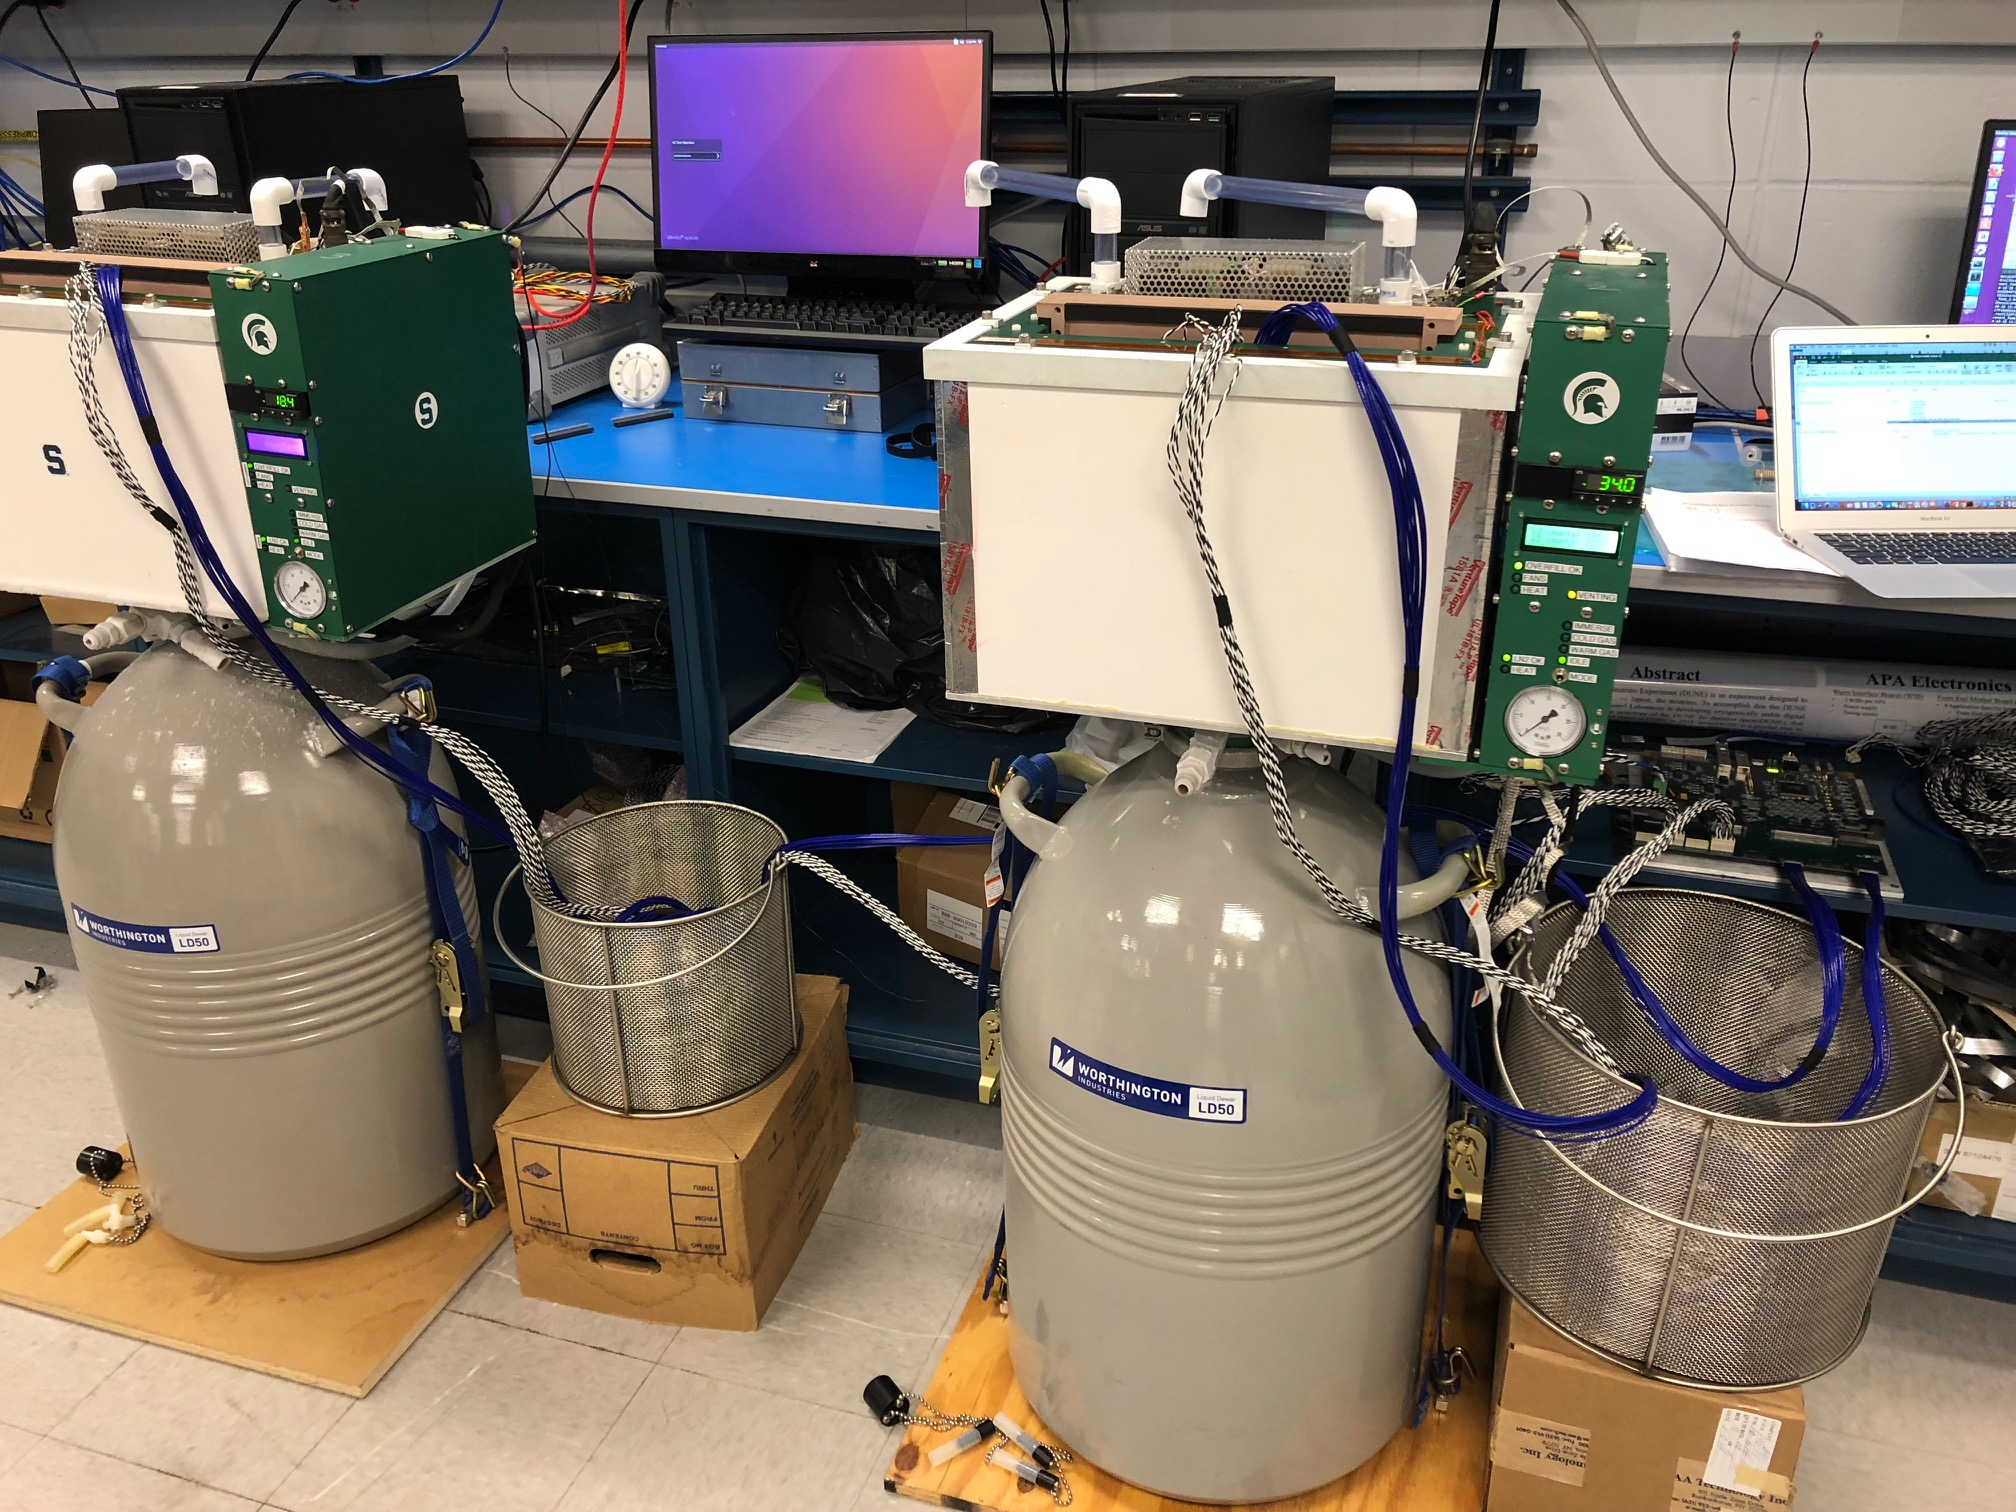
\includegraphics[width=0.4\linewidth]{sp-tpcelec-CTS2.jpeg}
\end{dunefigure}


%%%%%%%%%%%%%%%%%%%%%%%%%%%%%%%%%%%
%\subsection{Integrated Test Facilities}
%\label{sec:fdsp-tpcelec-qa-facilities}

The investigation of the system issues that can arise from the interaction 
of different detector components requires that a full system test of a slice
of the entire detector is performed. These tests are performed with \dwords{femb}
attached to \dword{apa}s enclosed in a structure that provides the same
grounding environment planned for the final \dword{dune} detector. The
power, control, and readout connections for the readout of the detector
will be provided using cryostat penetrations similar to the \dword{dune}
design. Prototypes of the final \dword{daq} will be used for readout and
control of the detector, and if possible the \dword{pds} and \dword{cpa}
detector components. We have identified three such system test stands
that we can use for system tests: the \dword{protodune} facility at CERN, the
\dword{iceberg} facility at \dword{fnal}, and the \num{40}\,\% \dword{apa} at \dword{bnl}.
We discuss these three setups in the following.


%%%%%%%%%%%%%%%%%%%%%%%%
\subsubsection{Photon Detectors}

\dword{pd} modules will arrive %at the \dword{itf} 
in custom crates.  Each crate will contain the ten modules required for one \dword{apa}, each individually packaged in a static-resistant sealed plastic bag, filled with clean dry nitrogen. Each \dword{pd} module is initially removed from its shipping bag, inspected visually, then (if it passes inspection) loaded into the optical scanner for operational testing.

%Before each \dword{pd} is integrated into an \dword{apa}, it is removed from its shipping bag and inspected visually. Modules passing this initial inspection are then loaded into the optical scanner for operational testing.

%The \dword{pd} optical scanner tests the operation of the photosensor readout chain to ensure all electrical connections are operational and also measures light-collection performance at several positions along the length of the module.  Duplicate identical optical scanners are used at the module assembly facility, where a scan is the last \dword{qc} test before the module is shipped to the \dword{itf}; the module is tested again immediately before installation, allowing a sensitive test for any changes in module performance due to shipping or storage.  This technique was used successfully in \dword{pdsp}, and will be replicated for \dword{dune}.
The optical scanner tests the operation of the photosensor readout chain to ensure all electrical connections are operational and measures light-collection performance at several positions along the length of the module.  Identical optical scanners are used at the module assembly facility, to test the module just before shipping. The test in the underground area %at the \dword{itf} 
will detect any changes in performance due to shipping or storage.  This technique was used successfully in \dword{pdsp}.

%The optical scanner consists of a light-tight box, approximately \num{2.5}m long, with a \num{0.75} $\times$ \num{0.75}m cross section. The box is fabricated of aluminum and acts as a Faraday cage to minimize electrical interference with measurements. In the \dword{dune} configuration, two \dword{pd} modules to be tested are inserted into the station through slots on the face of the box, guided by support rails of the type used in the \dword{apa}s, representing a final mechanical check of the dimensions of the module.  Electrical connection to the module uses an electrical connector identical to the ones in the \dword{apa} frames, allowing a final check of that crucial interface.Following insertion into the scanner, the insertion slots are closed and optically sealed, and the scan begins.\dword{dune} \dword{pd} readout electronics are used to bias and read out the module photosensors, while a UV LED is scanned along the length of the modules by an automated stepper-motor driven translation stage.  Measurements of the detector responses are made at 16 positions along the length of the module (on two sides for double-sided \dword{pd} modules), checking the performance of each of the dichroic filters.The response is compared to that measured in the assembly facility. Figure \ref{fig:fdsp-tc-pds-scanner} shows the scanner used to test the \dword{pdsp} photon detectors.
The optical scanner consists of a light-tight aluminum box, approximately \SI{2.5}{m} long, with a \num{0.75} $\times$ \num{0.75}m cross section. The box acts as a Faraday cage to minimize electrical interference with measurements. In the \dword{dune} test configuration, two \dword{pd} modules are inserted through slots on the face of the box, guided by support rails of the type used in the \dword{apa}s, which provides a final mechanical check of the \dword{pd} module dimensions.  The insertion slots are closed and optically sealed. 

The \dword{pd} module uses an electrical connector identical to the ones in the \dword{apa} frames, and that important interface is also checked in the scanner.  
Once the scan begins, \dword{dune} \dword{pd} readout electronics is used to bias and read out the photosensors, while a UV \dword{led} is scanned along the length of the modules via an automated stepper-motor driven translation stage.  Measurements are made at 16 positions along the length (on two sides for double-sided \dword{pd} modules), checking the performance of each  dichroic filter. The response is compared to that measured earlier at the assembly facility. Figure \ref{fig:fdsp-tc-pds-scanner} shows the scanner used to test the \dword{pdsp} \dwords{pd}.

\begin{dunefigure}[Photon detector scanner used for \dword{pdsp}]{fig:fdsp-tc-pds-scanner}
{Picture of the \SI{2.5}{m} long scanner used for operational tests of the \dword{pdsp} \dword{pd} modules prior to insertion into an \dword{apa}.} 

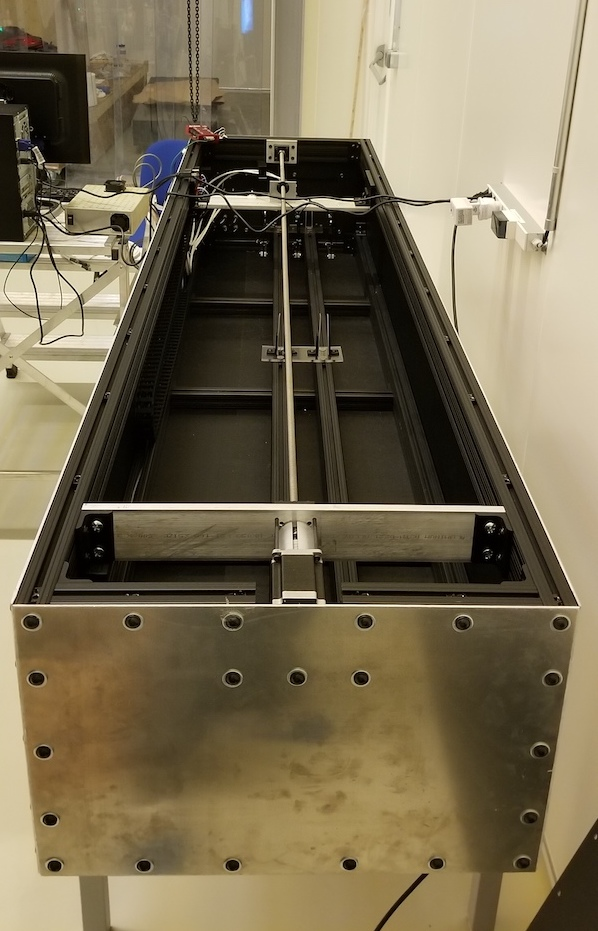
\includegraphics[height=.60\textheight, angle=0]{pds-scanner}
%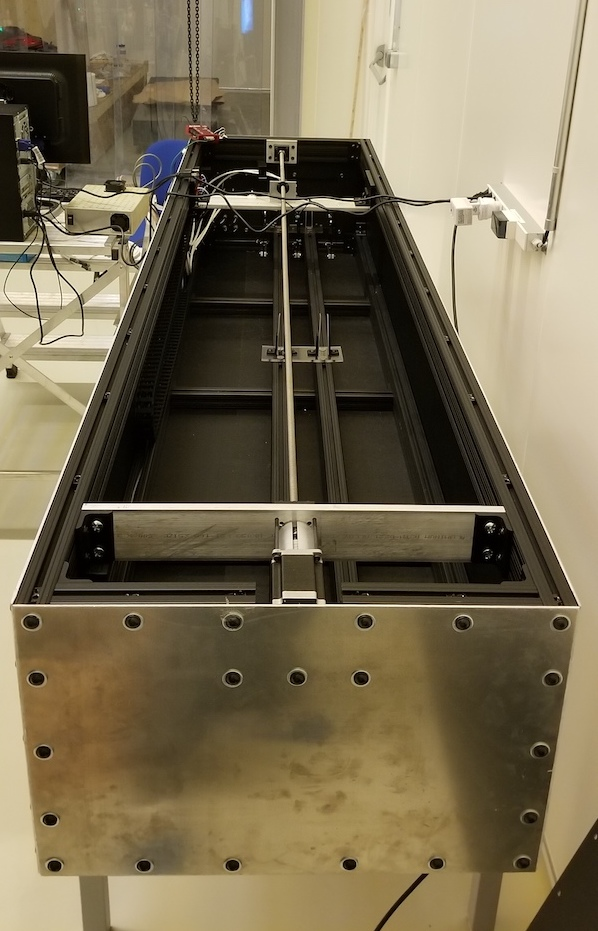
\includegraphics[width=1.0\textwidth, angle=-90]{pds-scanner}
\end{dunefigure}
\

%Photon detector are inserted into the \dword{apa}s immediately follows optical scanning.  Modules are inserted onto the \dword{pd} support rails; the connection to the cable harness, which is pre-installed in the \dword{apa} before wire wrapping, is automatic as the module is inserted.   Immediately after the module is inserted, an electrical continuity check ensures continuity between the \dword{pd} module and the \dword{pd} cable end connector where it exits the end of the \dword{apa}.

Following the optical scan, the \dword{pd} modules are inserted into an  \dword{apa} on a set of   support rails. The connection to the cable harness, which is pre-installed in the \dword{apa} before wire wrapping, is automatic. An electrical continuity check follows insertion to verify  continuity between the \dword{pd} module and the \dword{pd} cable end connector at the end of the \dword{apa}.

%%%%%%%%%%%%%%%%%%%%%%%%%%%%
%\subsection{Building Requirements and Infrastructure}
\subsection{Infrastructure Requirements}% for the ITF}

\label{sec:fdsp-tc-itf-req}
%The \dword{itf} building requirements are summarized in DocDb 11500.\cite{bib:docdb11500} The building to be used as the \dword{itf} has not yet been designated. To help identify or design the \dword{itf} building, a set of requirements were drafted. The requirements document defines the spaces needed for integration work but does not specify the final layout of the cleanroom. This will allow cleanroom spaces to be configured as part of building footprints as candidate buildings are identified. Because the building has not been designated, the cleanroom layout shown in Figure \ref{fig:fdsp-tc-itf-clean} should be taken as a concept; the final layout may change depending on the footprint of the building chosen as the \dword{itf}. The building requirements document\cite{bib:docdb11500}  defines the minimum spaces needed for all operations inside the \dword{itf} cleanroom. It also defines the space needed for the coldbox and the related cryogenic system, and it provides guidance for the space needed for material storage outside the cleanroom. It also establishes requirements for power and other general needs. Some requirements depend on the location of the building and the facilities available in the area. For example, office space for 20 scientists working in the \dword{itf} will be needed in the area but would not necessarily need to be in the \dword{itf} building itself if other local options are available. Some local machining facilities also fall into this category. 

The cleanroom requirements define the minimum space dimensions needed for integration work.  %The actual cleanroom configurations will depend on identified candidate buildings.  
Figure \ref{fig:fdsp-tc-itf-clean} illustrates a layout concept. Other requirements define the space needed for the \coldbox and  associated cryogenics system, provide guidance for material storage outside the cleanroom, and address  power and general infrastructure. 
 
%%%%%%%%%%%%%%%%%%%%%%%%%%%%
\subsection{Safety}
\label{sec:fdsp-tc-itf-safety}

Information on \dword{itf} safety is identical to what is listed in Section~\ref{sec:fdsp-tc-log-safety} because the underground area %\dword{itf} 
is operated by \dword{sdsd} as a Fermilab facility.    %If the \dword{itf} and %logistics facility \dword{sdwf} are near each other, the two sites can share one safety officer.    

%%%%%%%%%%%%%%%%%%%%%%%%%%%%
%\subsection{Cost, Schedule and Risk Analysis}   MOVED TO NEW FILE